\documentclass{SKP-beamer}

% --------------------------------------------------- %
\title[Cloud File Security]{Cloud Based File Security System with Hybrid Encryption}
\subtitle{PPD-II Second Review \hspace{0.3cm} | \hspace{0.3cm} PID: 23CSEP03}
\author[23CSEP03]{PID: 23CSEP03 \\[0.3cm] \small{Ashish Kumar (2301341013)} \\[0.1cm] \small{Ashish Singh (2301341014)} \\[0.1cm] \small{Avee Ranjan (2301341016)} \\[0.1cm] \small{Ayshi Shannidhya Panda (2301341017)} \\[0.3cm] \small{Under the guidance of} \\ \textbf{Mrs. Snehanjali Pradhan}}
\institute[SIT]{
  Silicon Institute of Technology
}
\date{October 2026}
\logo{

\includegraphics[scale=0.2]{sitlogo.png}
}
\subject{Cloud Based File Security System with Hybrid Encryption -- PPD-II Second Review}

% --------------------------------------------------- %
\begin{document}

\begin{frame}
  \titlepage
\end{frame}

% =================== OUTLINE =================== %
\begin{frame}{Outline}
\begin{enumerate}
  \item System / Design Development
  \item Implementation Progress
  \item Technical Approach
  \item Preliminary Results
  \item References
\end{enumerate}
\end{frame}

% ============================================================ %
%       SECTION 1: SYSTEM / DESIGN DEVELOPMENT                 %
% ============================================================ %
\section{System / Design Development}

\begin{frame}{System Overview --- CloudVault}
\begin{itemize}
  \item A cloud file storage system with \alert{hybrid encryption} (AES + RSA)
  \item Files are encrypted on the server during upload
  \item Files are decrypted \textbf{in the browser} during download
  \item User's RSA private key \alert{never leaves the browser}
  \item \textbf{Zero-effort sharing}: server re-wraps the AES key for the recipient
\end{itemize}
\end{frame}

\begin{frame}[fragile]{System Architecture}
\begin{block}{Three-Tier Design}
\small
\begin{tabular}{@{}ll@{}}
\textbf{Frontend} & React + Vite, Web Crypto API, Axios \\[0.3em]
\textbf{Backend} & Spring Boot 3 (Java 17), Spring Security, JPA \\[0.3em]
\textbf{Storage} & H2 Database + Encrypted Files on Disk \\
\end{tabular}
\end{block}

\vspace{0.3cm}

\begin{block}{Key Design Decisions}
\begin{itemize}
  \item \textbf{Key Envelope Table}: per-file, per-user encrypted AES key entries (OWNER / SERVER / SHARED)
  \item Server holds its \textbf{own RSA key pair} to enable sharing without involving the owner
  \item Encrypted AES key and IV sent via \textbf{custom HTTP headers} during download
\end{itemize}
\end{block}
\end{frame}

\begin{frame}{Database Design}
\begin{block}{Three Core Entities}
\begin{itemize}
  \item \textbf{User}: username, email, password hash (BCrypt), RSA public key (Base64)
  \item \textbf{EncryptedFile}: original filename, stored filename (UUID), file size, content type, IV, owner ID
  \item \textbf{FileKeyEntry}: file ID, user ID, encrypted AES key, key type (OWNER / SERVER / SHARED)
\end{itemize}
\end{block}

\vspace{0.2cm}
\begin{alertblock}{Access Control}
Each file has per-user encrypted AES key entries. Adding a user = creating a new key entry. Revoking access = deleting their key entry.
\end{alertblock}
\end{frame}

% ============================================================ %
%       SECTION 2: IMPLEMENTATION PROGRESS                     %
% ============================================================ %
\section{Implementation Progress}

\begin{frame}{What Has Been Completed}
\begin{block}{Backend (Spring Boot)}
\begin{itemize}
  \item \textbf{User Authentication}: Registration with RSA public key, login with JWT, BCrypt password hashing
  \item \textbf{Encryption Engine}: AES-256-GCM file encryption, RSA-2048-OAEP key wrapping using Java Cryptography Architecture
  \item \textbf{File Upload \& Storage}: Encrypted upload, UUID-based storage on disk, Key Envelope Table (OWNER + SERVER entries)
  \item \textbf{File Download}: Returns encrypted file + encrypted AES key + IV via custom HTTP headers
  \item \textbf{File Deletion}: Owner-only deletion with cleanup of disk file, key entries, and DB record
\end{itemize}
\end{block}
\end{frame}

\begin{frame}{What Has Been Completed (cont'd)}
\begin{block}{Frontend (React + Vite)}
\begin{itemize}
  \item \textbf{RSA Key Generation}: Web Crypto API generates RSA-2048 key pair in browser; private key stored in IndexedDB
  \item \textbf{Login \& Register Pages}: Dark-mode glassmorphism UI with form validation
  \item \textbf{Dashboard}: Tabbed file manager (My Files / Shared With Me) with stat cards
  \item \textbf{File Upload}: Drag-and-drop with circular progress indicator and 50MB size check
  \item \textbf{Client-Side Decryption}: Full pipeline --- RSA decrypt AES key $\rightarrow$ AES decrypt file $\rightarrow$ browser download
\end{itemize}
\end{block}
\end{frame}

\begin{frame}{Next Steps --- File Sharing}
\begin{block}{Sharing Module (To Be Implemented)}
\begin{itemize}
  \item \textbf{Share File}: Server decrypts AES key using its RSA private key, re-encrypts with recipient's RSA public key, stores SHARED key entry
  \item \textbf{Revoke Access}: Delete recipient's key entry from the database
  \item \textbf{Share Modal UI}: Enter recipient username, view shared users list, one-click revoke
\end{itemize}
\end{block}

\vspace{0.3cm}
\begin{exampleblock}{Why Sharing is the Final Step}
The encryption engine, key management, and file upload/download are already complete. Sharing simply \textbf{re-uses} the existing key wrapping infrastructure to create a new key entry for the recipient.
\end{exampleblock}
\end{frame}

% ============================================================ %
%       SECTION 3: TECHNICAL APPROACH                          %
% ============================================================ %
\section{Technical Approach}

\begin{frame}{Why Hybrid Encryption?}
\begin{itemize}
  \item \textbf{AES alone}: Fast for large files, but \alert{key distribution is insecure}
  \item \textbf{RSA alone}: Secure key exchange, but \alert{too slow for large files}
  \item \textbf{Hybrid}: AES-256 encrypts the file (fast) + RSA-2048 wraps the AES key (secure)
\end{itemize}
\end{frame}

\begin{frame}{Encryption Workflow}
\begin{center}
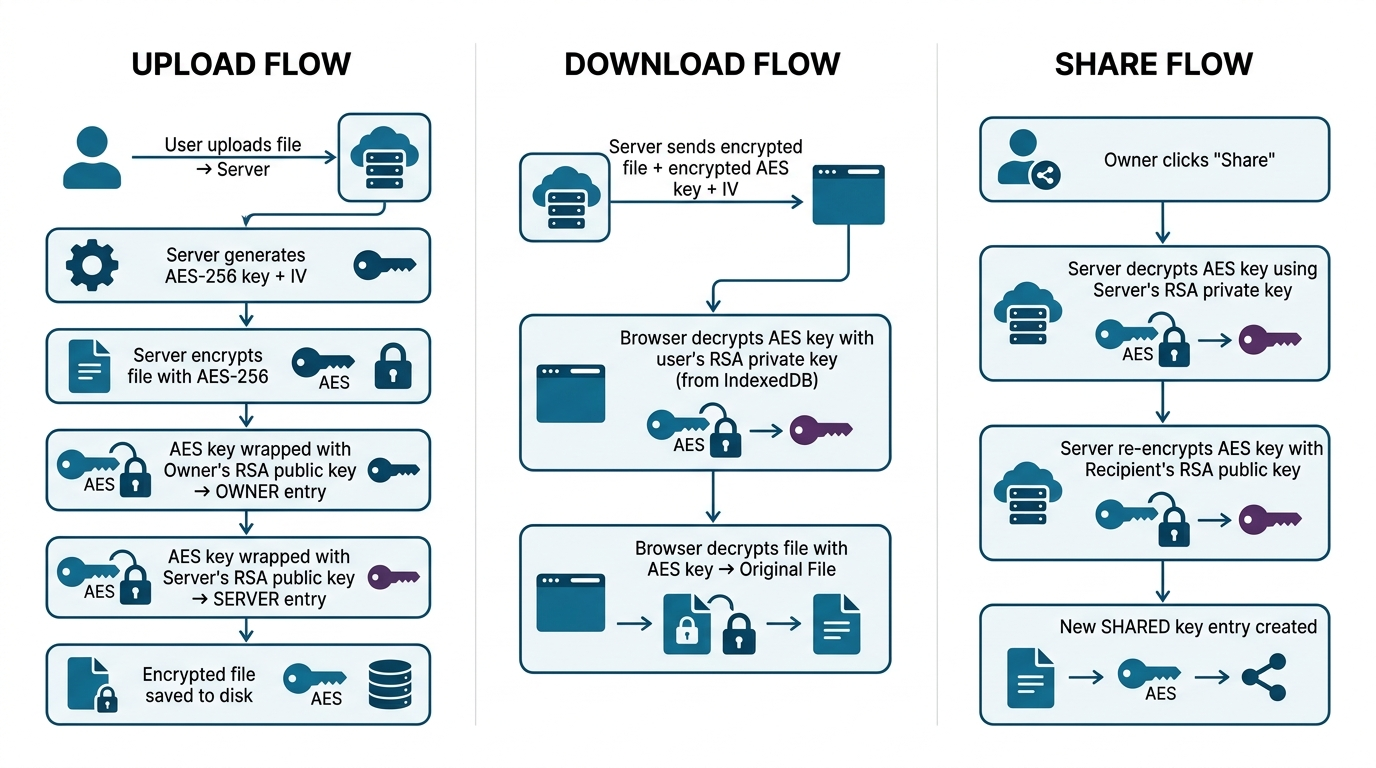
\includegraphics[width=\textwidth,height=0.78\textheight,keepaspectratio]{workflow.jpg}
\end{center}
\end{frame}

\begin{frame}{Security Layers}
\begin{block}{Multi-Layer Security}
\small
\begin{tabular}{@{}ll@{}}
\textbf{Passwords} & BCrypt hashing with random salt \\[0.2em]
\textbf{Sessions} & Stateless JWT tokens (24h expiry) \\[0.2em]
\textbf{API Protection} & Spring Security filter + JWT validation \\[0.2em]
\textbf{Files at Rest} & AES-256-GCM encrypted on disk \\[0.2em]
\textbf{Key Protection} & RSA-wrapped AES keys per user \\[0.2em]
\textbf{Client Keys} & RSA key pair stored in browser IndexedDB \\[0.2em]
\textbf{Server Keys} & RSA key pair stored as files on disk \\
\end{tabular}
\end{block}
\end{frame}

% ============================================================ %
%       SECTION 4: PRELIMINARY RESULTS                         %
% ============================================================ %
\section{Preliminary Results}

\begin{frame}{Functional Verification}
\begin{block}{Test Results (Completed Features)}
\small
\begin{tabular}{@{}lll@{}}
\textbf{Test Case} & \textbf{Status} & \textbf{Observation} \\[0.2em]
User Registration (RSA keygen) & \checkmark & Key pair generated in browser \\
User Login (JWT flow) & \checkmark & Token stored, API access works \\
File Upload (AES encryption) & \checkmark & Encrypted file stored on disk \\
File Download (client decrypt) & \checkmark & Original file recovered \\
File Deletion (owner only) & \checkmark & Disk + DB cleaned up \\
Unauthorized access & \checkmark & Returns 401, redirects to login \\
\end{tabular}
\end{block}

\vspace{0.2cm}
\begin{alertblock}{Pending Tests}
File sharing and access revocation tests will be conducted after the sharing module is implemented.
\end{alertblock}
\end{frame}

\begin{frame}{Demo --- Login \& Registration}
\vspace{-0.3cm}
\begin{columns}
\begin{column}{0.48\textwidth}
\begin{center}
\textbf{Login Page}\\[0.1cm]
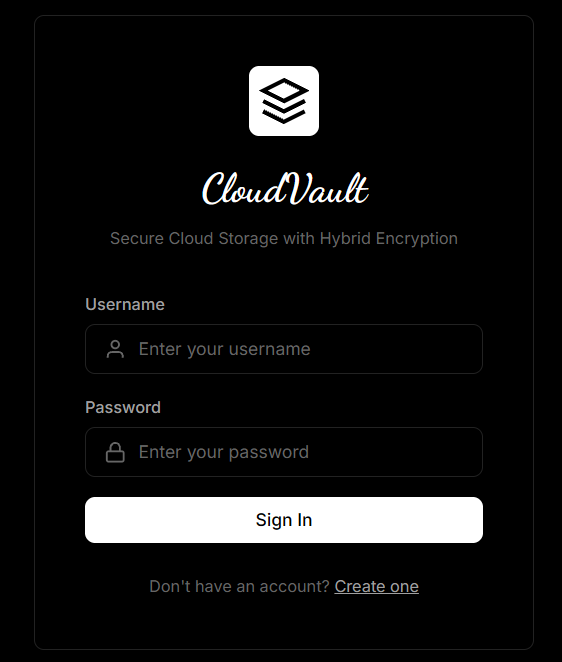
\includegraphics[width=\textwidth,height=0.55\textheight,keepaspectratio]{images/screenshot_login.png}
\end{center}
\end{column}
\begin{column}{0.48\textwidth}
\begin{center}
\textbf{Register Page}\\[0.1cm]
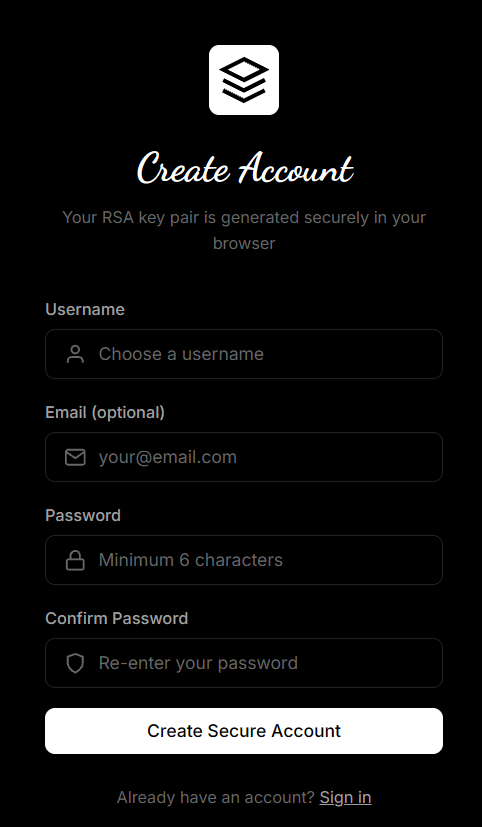
\includegraphics[width=\textwidth,height=0.55\textheight,keepaspectratio]{images/screenshot_register.png}
\end{center}
\end{column}
\end{columns}
\end{frame}

\begin{frame}{Demo --- Dashboard}
\vspace{-0.3cm}
\begin{center}
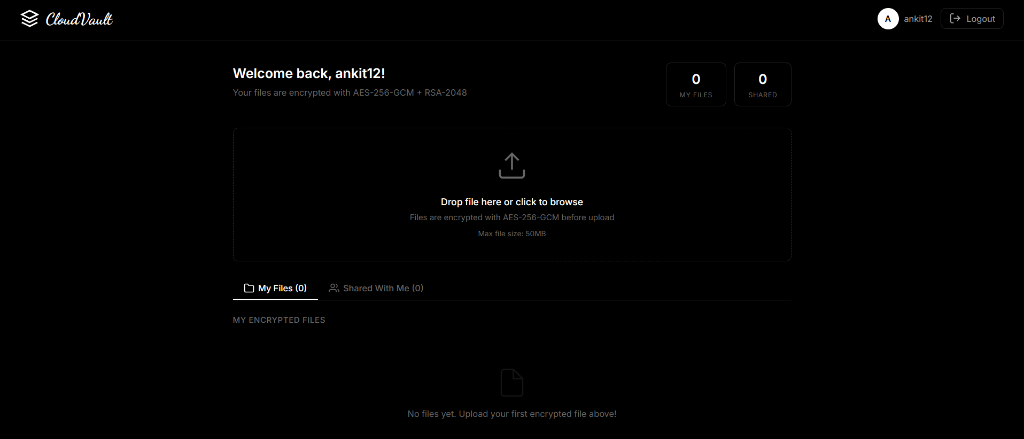
\includegraphics[width=\textwidth,height=0.65\textheight,keepaspectratio]{images/screenshot_dashboard.png}
\end{center}
\end{frame}

% =================== 5: REFERENCES =================== %
\section{References}
\begin{frame}{References}
    \nocite{*}
	\bibliography{reference}
	\bibliographystyle{unsrt}
\end{frame}

% =================== THANK YOU =================== %
\begin{frame}{}
\begin{center}
\vspace{2cm}
{\Huge \textbf{Thank You}}
\end{center}
\end{frame}

\end{document}
